% SCENE NATIGATION

Following is a list o scene navigation solutions.
Each one can contribute to a more powerful and easy interface.


\subsubsection{Smart and Physically Based Camera, 2006}

In order to ensure users not ``getting lost'' in the virtual space,
Buchholz, Bohnet and D�llner \cite{SMARTCAM}
propose a camera that is is both smart and physically-based.
Smart in the sense that it is aware of confusing,
disorienting viewing situations, providing means to circumvent them.
Physically based because it is supported by a physics model of 3D motion
to ensure steady, continuous user movements.

In order to solve the disorientation problem, the camera must identify situations
when to intervene.
For that matter a metric, called orientation value, was created.
Each view is classified by counting its pixels, granting each one a different value:
landmarks are granted the highest values; terrain gets high values and sky gets low values.
A threshold can then be established and views below it are classified ``disoriented''.

When such an event takes place, smart navigation techniques restrict camera control.
The constraints posed to user control must be as comprehensible as possible.
Camera movement should also be time-coherent and physically sound.

The maintenance strategy solves critical situations such as (see Fig.\ref{FIG-SMARTCAM1}, left):

\begin{enumerate}[a)]
	\item The user rotates the flight direction and causes the camera to look too far beyond the terrain border.
		The rotation is accepted but outweighed by a slight rear movement away from the border.
	\item The user is flying forward beyond the terrain border.
		The maintenance strategy temporarily tilts down the view direction until a maximum angle is reached.
	\item If no more tilting is possible, the strategy rotates the flight direction parallel to the terrain
		to fly along the terrain border.
\end{enumerate}

\begin{figure}[!ht]
	\centering
	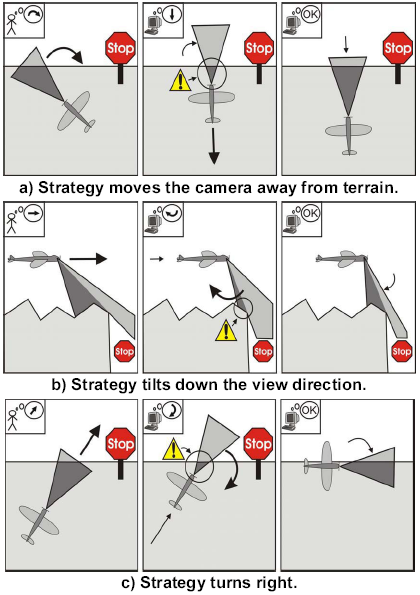
\includegraphics[height=7cm]{gfx/smartcam05-1.png}
	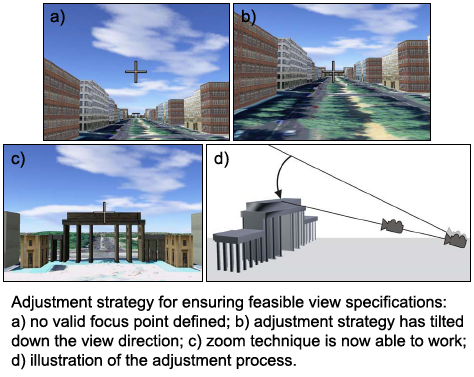
\includegraphics[height=5cm]{gfx/smartcam05-2.png}
	\caption{SPB Cam: Maintenance strategy for keeping high orientation values (left); Adjustment strategy for ensuring of feasible view specifications (right).}
	\label{FIG-SMARTCAM1}
\end{figure}

\paragraph{Discussion}
\label{sec:Paragraph}

A camera system such as this can be useful aiding non-experienced users such as clients in navigation tasks
since it maintains useful landmarks in the user's view.
The physically-based engine would grant additional realism to the navigation experience, providing collision
detection, inertia and a spring behavior that would soften the user trajectories.


\subsubsection{Speed-dependent Automatic Zooming, 2000}

Igarashi and Hinckley \cite{SPEEDZOOM} propose a simple idea for scrolling through large areas of information.
The speed at which the scrolling occurs changes the zooming of the area seen.
This makes sense since the faster the area is scrolling, the longer ahead the user needs to see.

\paragraph{Discussion}
\label{sec:Paragraph}

This could be easily applied to birds'-eye-view maps of large areas.
The scrolling of the map by the user would then trigger different zooming factors depending on the scrolling speed,
improving the navigation and exploration of the map.


% TODO: \cite{EXPLORE3D}


\subsubsection{Path Drawing for 3D Walkthrough, 1998}

Igarashi et al. \cite{PATH3D} start by identifying the main two types of walkthrough techniques:
\emph{driving}, where the user continuously changes camera position with move and rotation buttons and
\emph{flying}, where the user picks the target location with a pointing device and a trajectory is calculated
and animated from the starting position to the picked one.

Each of them have disadvantages: driving requires the user to control the trajectory all the way until arriving
at the destination -- during this time the controlling is hard if the system faces slow refreshing times;
flying lacks expressive power since the user can't control the path neither the final orientation.

The proposed solution is an extension of the flying technique: the user draws the desired path he wants to take
on the screen. It gets projected onto the walking surfaces and the generated path is animated. During the animation
the user faces the tangential direction related to the path.
This brings the additional advantage of the user being able to define where he will be facing at the end of the
animation.

This technique can be used is two different ways.
The user can draw a long stroke specifying the path at once or he can draw successions of small strokes.

As limitations the authors state the path expressiveness being limited to the walking surface planes and
the need for the user's avatar to be present on the view if one wants to draw the path from the user's feet.
 

\begin{figure}[!ht]
	\centering
	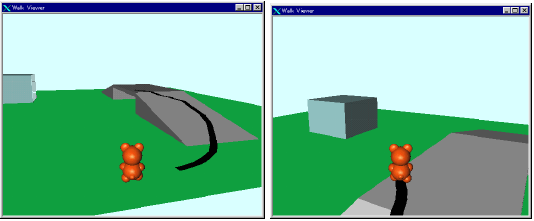
\includegraphics[width=12cm]{gfx/path3d.png}
	\caption{One long path and one short one}
	\label{FIG-PATH3D}
\end{figure}

\paragraph{Discussion}
\label{sec:Paragraph}

This navigation mode could be handy in the review scenario.
The only disadvantage found is the need to see the user's avatar for the mapping to be perfect.